\section{String Matching}

\subsection{The naive string-matching algorithm}

\begin{description}
\descitem{32.1-1} \textit{Show the comparisons the naive string matcher makes for the pattern $P = 0001
$ in the text $T = 000010001010001$.}

\begin{ex}
    \begin{figure}[H]
      \centering
      \begin{subfigure}[t]{.45\textwidth}
        \centering
        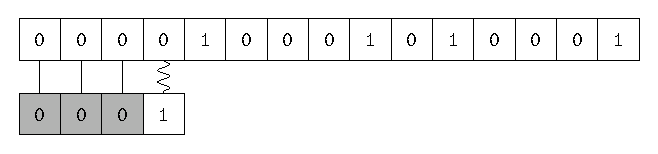
\includegraphics[scale=.6]{img/32_1-1/32_1-1_1.pdf}
        \caption{$\texttt{shift} = 0$}\label{fig:32_1-1_1}
      \end{subfigure}
      \begin{subfigure}[t]{.45\textwidth}
        \centering
        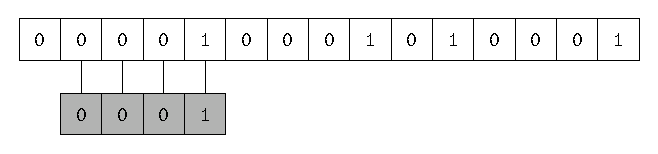
\includegraphics[scale=.6]{img/32_1-1/32_1-1_2.pdf}
        \caption{$\texttt{shift} = 1$}\label{fig:32_1-1_2}
      \end{subfigure}
      \begin{subfigure}[t]{.45\textwidth}
        \centering
        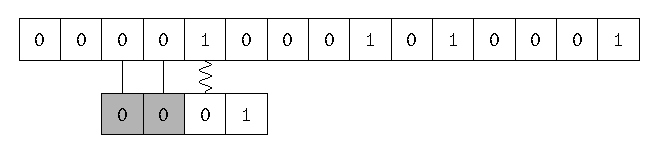
\includegraphics[scale=.6]{img/32_1-1/32_1-1_3.pdf}
        \caption{$\texttt{shift} = 2$}\label{fig:32_1-1_3}
      \end{subfigure}
      \begin{subfigure}[t]{.45\textwidth}
        \centering
        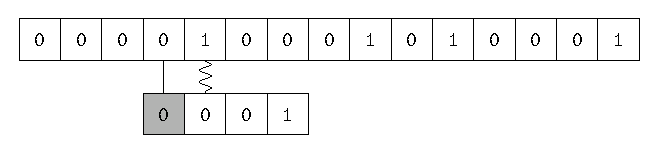
\includegraphics[scale=.6]{img/32_1-1/32_1-1_4.pdf}
        \caption{$\texttt{shift} = 3$}\label{fig:32_1-1_4}
      \end{subfigure}
      \begin{subfigure}[t]{.45\textwidth}
        \centering
        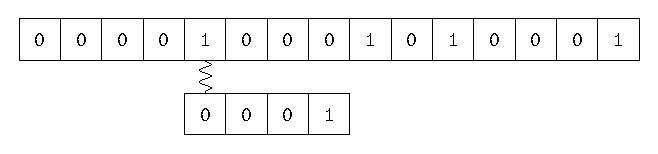
\includegraphics[scale=.6]{img/32_1-1/32_1-1_5.pdf}
        \caption{$\texttt{shift} = 4$}\label{fig:32_1-1_5}
      \end{subfigure}
      \begin{subfigure}[t]{.45\textwidth}
        \centering
        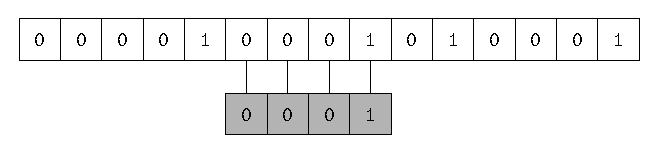
\includegraphics[scale=.6]{img/32_1-1/32_1-1_6.pdf}
        \caption{$\texttt{shift} = 5$}\label{fig:32_1-1_6}
      \end{subfigure}
      \begin{subfigure}[t]{.45\textwidth}
        \centering
        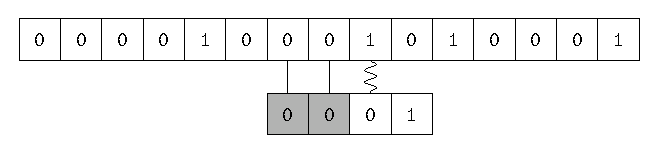
\includegraphics[scale=.6]{img/32_1-1/32_1-1_7.pdf}
        \caption{$\texttt{shift} = 6$}\label{fig:32_1-1_7}
      \end{subfigure}
      \begin{subfigure}[t]{.45\textwidth}
        \centering
        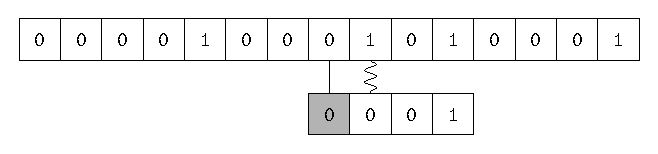
\includegraphics[scale=.6]{img/32_1-1/32_1-1_8.pdf}
        \caption{$\texttt{shift} = 7$}\label{fig:32_1-1_8}
      \end{subfigure}
      \begin{subfigure}[t]{.45\textwidth}
        \centering
        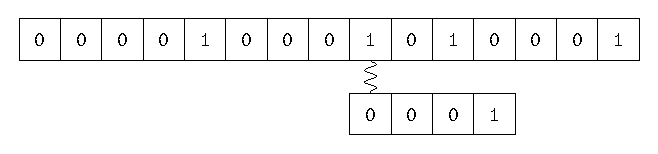
\includegraphics[scale=.6]{img/32_1-1/32_1-1_9.pdf}
        \caption{$\texttt{shift} = 8$}\label{fig:32_1-1_9}
      \end{subfigure}
      \begin{subfigure}[t]{.45\textwidth}
        \centering
        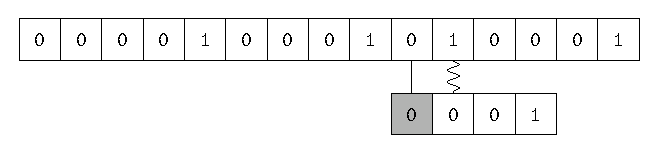
\includegraphics[scale=.6]{img/32_1-1/32_1-1_10.pdf}
        \caption{$\texttt{shift} = 9$}\label{fig:32_1-1_10}
      \end{subfigure}
      \begin{subfigure}[t]{.45\textwidth}
        \centering
        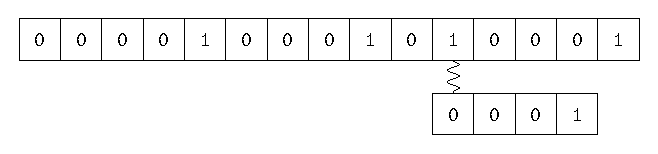
\includegraphics[scale=.6]{img/32_1-1/32_1-1_11.pdf}
        \caption{$\texttt{shift} = 10$}\label{fig:32_1-1_11}
      \end{subfigure}
      \begin{subfigure}[t]{.45\textwidth}
        \centering
        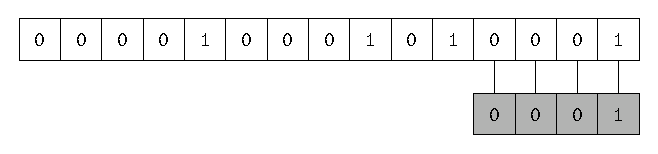
\includegraphics[scale=.6]{img/32_1-1/32_1-1_12.pdf}
        \caption{$\texttt{shift} = 11$}\label{fig:32_1-1_12}
      \end{subfigure}
      \caption{Recherche de la sous châine $0001$ dans $000010001010001$ avec l'algorithme naïve.} 
      \label{fig:naive-match-string} 
    \end{figure}
\end{ex}


\descitem{32.1-2} \textit{Suppose that all characters in the pattern $P$ are different. Show how to accelerate
\proc{Naive-String-Matcher} to run in time $O(n)$ on an $n$-character text $T$.}

\begin{ex}
\begin{codebox}
\Procname{\algo{Naive-String-Matcher-Diff}$(\id{T}, \id{P})$}
    \li $n = \attrib{T}{length}$, $m = \attrib{P}{length}$, $s = 0$
    \li \While $\id{s} \le n -m$ \Do
    \li \If $P[1\twodots m] == T[s + 1\twodots s + m]$ \Then
    \li print "Pattern occurs with shift" s 
    \li $s \gets s + m$ 
    \li \Else 
    \li $s \gets s + 1$ \End
\end{codebox}
\end{ex}

\descitem{32.1-3} \textit{Suppose that pattern $P$ and text $T$ are randomly chosen strings of length $m$ and $n$,
respectively, from the $d$-ary alphabet $\Sigma_d = \{0, 1, \ldots, d-1\}$, where $d \ge 2$. Show
that the expected number of character-to-character comparisons made by the implicit loop in line $4$ of the naive algorithm is
    \[(n-m+1) \frac{1-d^{-m}}{1-d^{-1}} \le 2(n - m + 1)\]
over all executions of this loop. (Assume that the naive algorithm stops comparing
characters for a given shift once it finds a mismatch or matches the entire pattern.)
Thus, for randomly chosen strings, the naive algorithm is quite efficient.  }

\begin{exrev}

\end{exrev}

\descitem{32.1-4} \textit{Suppose we allow the pattern $P$ to contain occurrences of a gap character $\diamondsuit$ that
can match an \textit{arbitrary} string of characters (even one of zero length). For example,
the pattern $ab\diamondsuit ba\diamondsuit c$ occurs in the text $cabccbacbacab$ abstract as}

    $c\smallunderbrace{ab}_{ab}\smallunderbrace{cc}_{\diamondsuit}\smallunderbrace{ba}_{ba}\smallunderbrace{cba}_{\diamondsuit}\smallunderbrace{c}_{c}ab$

\textit{and as}

    $c\smallunderbrace{ab}_{ab}\smallunderbrace{ccbac}_{\diamondsuit}\smallunderbrace{ba}_{ba}\smallunderbrace{}_{\diamondsuit}\smallunderbrace{c}_{c}ab$.

\textit{Note that the gap character may occur an arbitrary number of times in the pattern
but not at all in the text. Give a polynomial-time algorithm to determine whether
such a pattern $P$ occurs in a given text $T$ , and analyze the running time of your
algorithm.}
\begin{ex}

\begin{codebox}
\Procname{\algo{Naive-String-Matcher-With-Gap}$(\id{T}, \id{P}, \id{gap})$}
    \li $n = \attrib{T}{length}$,  $m = \attrib{P}{length}$, $s = 0$
    \li \For each $P_i$ in partition $P$ delimited by $\id{gap}$ character \Do
    \li $m_i = \attrib{P_i}{length}$
    \li \While $s \le n - m_i$ \Do
    \li \If $P_i[1\twodots m_i] == T[s + 1\twodots s + m_i]$ \Then
    \li $\id{shift}[i] \gets s$
    \li \Break \End
    \li $s \gets s + 1$ \End \End
    \li \If $s \le n-m_{\text{last}}$ \Then
    \li print "Pattern occurs with shift" $\id{shift}[1]$ \End
\end{codebox}

Notons $p$ le nombre des patterns $P_i$, $m_{\min}$ et $m_{\max}$ les patterns $P_i$ respectivement plus court et plus long. 
Le \textit{parsing} des $P_i$ nécessite $O(m)$. Puis, en considérant le pseudocode, la recherche de pattern avec trou est en $O(p \cdot (n - m_{\min} + 1) \cdot m_{\max} + m)$. 

Supposons maintenant qu'il n'y a pas de $\diamondsuit$ consécutive dans $P$ et que les sous patterns sont de taille équitable, \textit{i.e.} $\forall i \le p, m_i = \frac{m - p + 1}{p}$. Alors, on a
    \[O(p \cdot (n - m_{\min} + 1) \cdot m_{\max} + m) = O (nm).\]

\end{ex}

\end{description}

\subsection{The Rabin-Karp algorithm}

\begin{description}
\descitem{32.2-1} \textit{Working modulo $q = 11$, how many spurious hits does the Rabin-Karp matcher encounter in the text $T = 3141592653589793$ when looking for the pattern $P = 26$?}
\begin{ex}
Trois, car $26 \equiv 15 \equiv 59 \equiv 92\mod 11$.
\end{ex}
\descitem{32.2-2} \textit{How would you extend the Rabin-Karp method to the problem of searching a text
string for an occurrence of any one of a given set of $k$ patterns? Start by assuming
that all $k$ patterns have the same length. Then generalize your solution to allow the
patterns to have different lengths.}

\begin{ex}
\begin{codebox}
%TODO:add time complexity
\Procname{\algo{Rabin-Karp-Matcher-$k$-Patterns-Same-Length}$(\id{T}, \id{P}, \id{k}, \id{d}, \id{q})$}
    \li $n = \attrib{T}{length}$,  $m = \attrib{P}{length}$, $h = d^{m-1} \mod q$, $t = 0$
    \li \For $i=0$ \To $k$ \Do
        \li $p[i] = 0$ \End
    \li \For $i=0$ \To $m$ \Comment Preprocessing \Do
      \li \For $j=0$ \To $k$ \Do
        \li $p[j] = (d \cdot p[j] + P[j][i]) \mod q$ \End
      \li $t = (d \cdot t + T[i]) \mod q$ \End
    \li \For $s = 0$ \To $n - m$ \Comment Matching \Do
      \li \For $j=0$ \To $k$ \Do
        \li \If $p[j] == t$ \Then
           \li \If $P[j][1 \twodots m] == T[s + 1 \twodots s + m]$ \Then
             \li print "Pattern" $P[j]$ "occurs with shift" $s$ 
           \End
        \End
      \End
      \li \If $s < n - m$ \Then
        \li $t = (d \cdot (t - T[s+1] \cdot h) + T[s + m + 1]) \mod q$
      \End
   \End
\end{codebox}
\begin{codebox}
\Procname{\algo{Rabin-Karp-Matcher-With-$k$-Patterns-Diff-Length}$(\id{T}, \id{P}, \id{k}, \id{d}, \id{q})$}
    \li $n = \attrib{T}{length}$
    \li \For $i=0$ \To $k$ \Do
        \li $p[i] = 0$ 
        \li $t[i] = 0$ 
        \li $m_i = \attrib{P[i]}{length}$
        \li $h[i] = d^{m_i - 1} \mod q$ 
    \End
    \li \For $i=0$ \To $m_{\max}$ \Comment Preprocessing \Do
      \li \For $j=0$ \To $k$ \Do
        \li \If $i < m_j$ \Then 
          \li $p[j] = (d \cdot p[j] + P[j][i]) \mod q$ 
          \li $t[j] = (d \cdot t[j] + T[i]) \mod q$ 
        \End
      \End
    \End
    \li \For $s = 0$ \To $n - m_{\min}$ \Comment Matching \Do
      \li \For $j=0$ \To $k$ \Do
        \li \If $p[j] == t$ \Then
           \li \If $P[j][1 \twodots m_j] == T[s + 1 \twodots s + m_j]$ \Then
             \li print "Pattern" $P[j]$ "occurs with shift" $s$ 
           \End
        \End
      \End
      \li \If $s < n - m_{\min}$ \Then
        \li \For $i=0$ \To $k$ \Do
          \li $t[i] = (d \cdot (t[i] - T[s+1] \cdot h[i]) + T[s + m[i] + 1]) \mod q$
        \End
      \End
   \End
\end{codebox}
\end{ex}

\descitem{32.2-3} \textit{}
\descitem{32.2-4} \textit{}
\end{description}

